
\chapter{Synthetic data sets}

\index{synthetic data set}

One very useful skill is the ability to quickly create \textit{synthetic}
(artificial; generated by your own code and random-number generators) data
sets that have certain properties. Sometimes we use such data to sanity check
the results of our code with ``idealistic'' (simplified and known) inputs.
Sometimes we use synthetic data as a baseline with which to compare real-world
data sets that we suspect have similar characteristics. And sometimes we
simply don't have access to relevant real-world data but we need inputs into
some simulation process.

\section{Random number generation}

\index{random number}
\index{seed (of a random number generator)}

\subsection{Setting the seed}

Generating \textbf{random number}s is an activity we perform surprisingly often
in Data Science. ``Random numbers,'' as it turns out, aren't truly random,
because the programming language uses a bizarre -- but deterministic and
repeatable -- algorithm to come up with them. This is nice, because we can
guarantee that each time we run a program we'll get the same sequence of random
numbers. We do this by setting the random number generator's \textbf{seed} to a
particular value. It helps us in debugging our code, because otherwise, a
shifting sequence of numbers would be a frustrating moving target. 

\texttt{seed@\texttt{seed()} (NumPy)}

NumPy provides a really nice library for all this, all of which is in the
namespace \texttt{np.random}. To set the random number generator's seed, all
you do is call its \texttt{seed()} function and pass it your favorite number:

\begin{Verbatim}[fontsize=\small,samepage=true,frame=single,framesep=3mm]
np.random.seed(13)
\end{Verbatim}

(I chose 13 because that was my little league baseball uniform number as a
kid.) I recommend you put this line of code (with any positive integer you
like) near the top of any \texttt{.py} file in which you do random number
generation. If you want a different sequence of random numbers later, you can
either change the integer to something different, or comment out the line
altogether by prepending a ``\texttt{\#}'' character.

\subsection{Generating random values}

To actually generate a random number value, you first have to figure out what
\textbf{distribution} you want it to come from. Think of a distribution as a
KDE from last chapter: it's a way of specifying which values will be more
likely to occur and which will be less likely. The two standard distributions
we'll use most are:

\begin{itemize}
\itemsep.1em
\item \textbf{Normal/Gaussian}. As mentioned on p.~\pageref{Gaussian}, a
``normal'' distribution is a standard bell curve with a central \textbf{mean}
and a \textbf{standard deviation} that determines how wide the curve is. The
Gaussian distribution with mean 65 and standard deviation 4 (perhaps
representing the speed of various cars on the highway) is shown on the top
half of Figure~\ref{distributions}.
\item \textbf{Uniform}. A uniform distribution specifies that every value
within a certain range (a \textbf{min} and a \textbf{max}) should be
\textit{equally likely}. An example for a min of 0 and a max of 60 (perhaps
representing the minute past the hour that various babies in a maternity ward
were born) is shown on the bottom of the same figure.
\end{itemize}

\begin{figure}[ht]
\centering
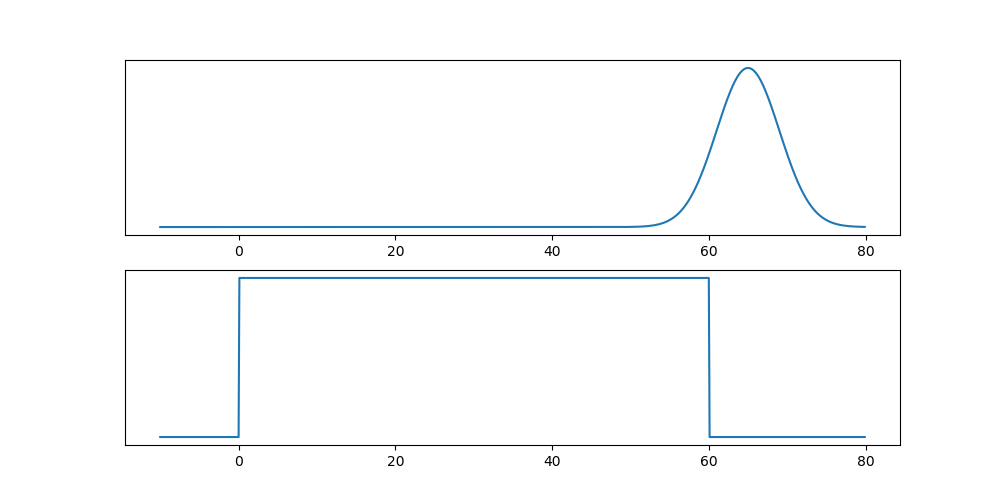
\includegraphics[width=1.0\textwidth]{distributions.png}
\caption{A normal, and uniform, distributions, shown as KDE-like curves.}
\label{distributions}
\end{figure}

If you're interpreting Figure~\ref{distributions} correctly, you can see that
if we generate random numbers from the top distribution, the majority will be
between 60-ish and 70-ish miles per hour, with many near 65 mph and almost
never anything lower than 50 or greater than 80. If we generate them from the
bottom distribution, however, the babies' birth minutes will all be between 0
and 60 but with no particular tendency towards any value in that range more
than any other.

Let's see if that works. The three arguments to \texttt{normal()} are (1) the
mean of the distribution, (2) the standard deviation, and (3) how many random
numbers you actually want. We'll just start with one at a time:

\begin{Verbatim}[fontsize=\small,samepage=true,frame=single,framesep=3mm]
np.random.seed(13)
print(np.random.normal(65,4,1))
\end{Verbatim}
\vspace{-.2in}

\begin{Verbatim}[fontsize=\small,samepage=true,frame=leftline,framesep=5mm,framerule=1mm]
[62.15043735]
\end{Verbatim}

\begin{Verbatim}[fontsize=\small,samepage=true,frame=single,framesep=3mm]
print(np.random.normal(65,4,1))
\end{Verbatim}
\vspace{-.2in}

\begin{Verbatim}[fontsize=\small,samepage=true,frame=leftline,framesep=5mm,framerule=1mm]
[68.01506551]
\end{Verbatim}

\begin{Verbatim}[fontsize=\small,samepage=true,frame=single,framesep=3mm]
print(np.random.normal(65,4,1))
\end{Verbatim}
\vspace{-.2in}

\begin{Verbatim}[fontsize=\small,samepage=true,frame=leftline,framesep=5mm,framerule=1mm]
[64.82198769]
\end{Verbatim}

\begin{Verbatim}[fontsize=\small,samepage=true,frame=single,framesep=3mm]
print(np.random.normal(65,4,1))
\end{Verbatim}
\vspace{-.2in}

\begin{Verbatim}[fontsize=\small,samepage=true,frame=leftline,framesep=5mm,framerule=1mm]
[66.80724935]
\end{Verbatim}

True to form. We keep getting numbers quite close to 65 mph, with a little bit
of variation. Note that if we reset the seed to our original value, our next
call to \texttt{normal()} gives an identical result to the first one, above:

\begin{Verbatim}[fontsize=\small,samepage=true,frame=single,framesep=3mm]
np.random.seed(13)
print(np.random.normal(65,4,1))
\end{Verbatim}
\vspace{-.2in}

\begin{Verbatim}[fontsize=\small,samepage=true,frame=leftline,framesep=5mm,framerule=1mm]
[62.15043735]
\end{Verbatim}

And of course it's easy to generate many speeds at a time (say, eight):

\begin{Verbatim}[fontsize=\small,samepage=true,frame=single,framesep=3mm]
print(np.random.normal(65,4,8))
\end{Verbatim}
\vspace{-.2in}

\begin{Verbatim}[fontsize=\small,samepage=true,frame=leftline,framesep=5mm,framerule=1mm]
[60.81849148 61.8440439  59.95357622 67.25138714 64.02669499 68.65496282
 66.26940369 65.50921312]
\end{Verbatim}

Notice that each time we call \texttt{normal()}, we get an array back (even if
it has only a single value).

By the way, we should sure expect that if we generate many random speeds, and
take their average, it should be darn close to 65 mph:

\begin{Verbatim}[fontsize=\small,samepage=true,frame=single,framesep=3mm]
print(np.random.normal(65,4,1000).mean())                        
\end{Verbatim}

\begin{Verbatim}[fontsize=\small,samepage=true,frame=leftline,framesep=5mm,framerule=1mm]
65.01577962051226
\end{Verbatim}

Yep.

